\chapter{Primeri}

\section{Primer za učenje jezikov}

\subsection{Opis problema}

DEFG je preprosta grafična aplikacija, ki uporabnikom olajša učenje tujih jezikov. Deluje na preprostem principu pomnjenja besed. Igralcu se na zaslonu pokaže beseda v domačem jeziku in tri besede v jeziku, ki se ga uporabnik skuša naučiti. Dve besedi od treh tujih sta naključno izbrani, tretja pa je pravilni odgovor.

V primeru pravilnega odgovora se uporabniku pokaže naslednja beseda in trije novi odgovori. Tako uporabnik nadaljuje z učenjem. Če uporabnik izbere napačni odgovor, se na zaslonu pojavi pravilni prevod besede, tako da se ima uporabnik možnost naučiti besedo. Ko si uporabnik ogleda pravilni odgovor se igra ponastavi ter začne od začetka.

Na sliki [\ref{german}] je glavni zaslon aplikacije s tremi možnimi odgovori.

\begin{figure}
\begin{center}
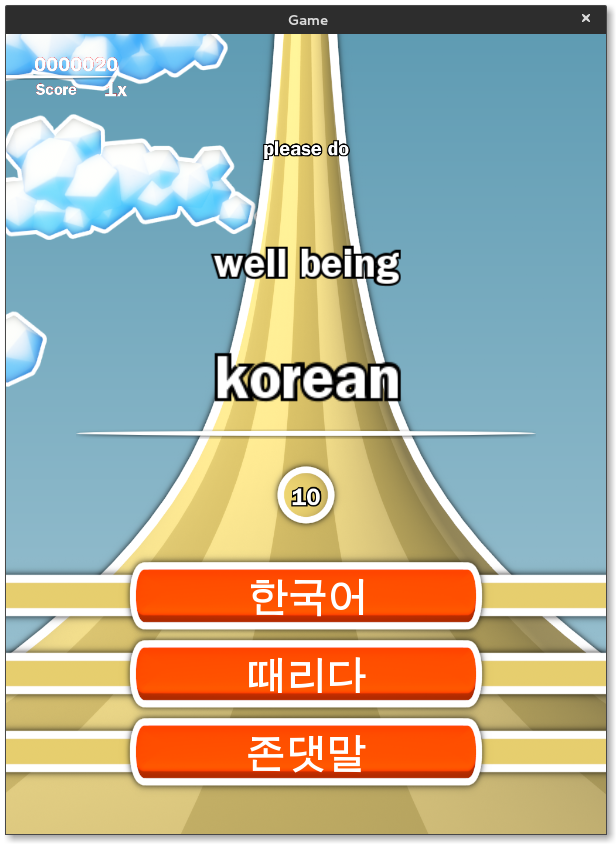
\includegraphics[width=5.5cm]{pic/defg-korean.png}
\end{center}
\caption{Primer delovanja Korejske verzije na namiznem računalniku}
\label{korean}
\end{figure} 


Ena izmed glavnih zahtev igre je izpis različnih pisav in posebnih znakov. Poleg prikazane verzije nemščina-angleščina, je bila aplikacija razvita tudi z idejo učenja jezikov, ki ne uporabljajo latinice. Slika [\ref{korean}] prikazuje primer učenja Korejščine. Aplikacije mora biti sposobna izrisovati velik nabor različnih abeced.

\begin{figure}
\begin{center}
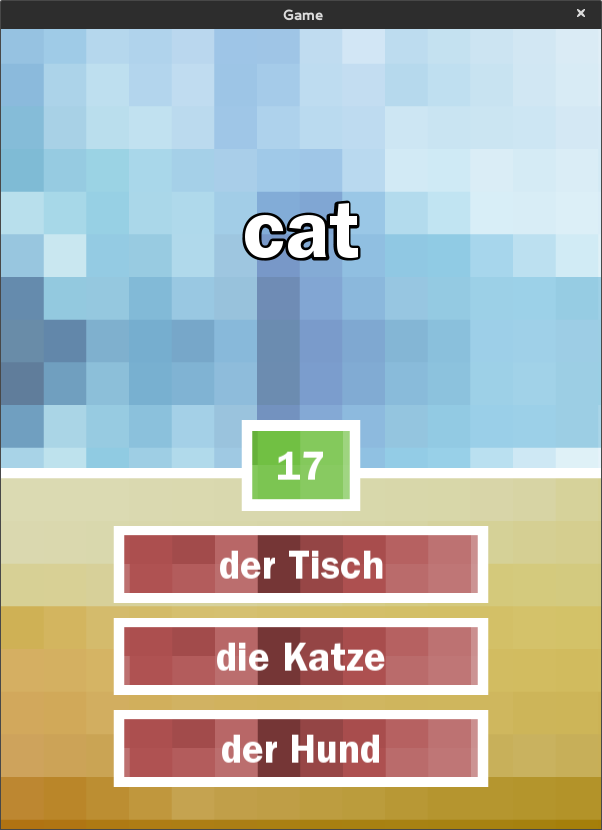
\includegraphics[width=5.5cm]{pic/defg-german.png}
\end{center}
\caption{Primer delovanja Nemške verzije na mobilni napravi}
\label{german}
\end{figure} 

Aplikacija je bila zamišljena kot mobilna aplikacijam za platformi iOS in Android, vendar kot smo že opisali je zelo uporabno imeti način razvoja na namiznem računalniku. Zaradi tega smo se odločili za metodo PlayN.

\subsection{Uporabljena metoda}

Izmed vseh obravnavanih metod se nam je zdela najbolj primerna metoda PlayN. Razlogi za izbiro PlayN so naslednji:

\begin{itemize}
\item PlayN je odprtokoden projekt. V primeru težav lahko pogledamo v izvorno kodo projekta in po potrebi nedelovanje spremenimo.
\item Licenca, ki jo PlayN uporablja, ni omejujoča in v primerjavi z nekaterimi plačljivimi metodami, ne zahteva nobenega plačila pred uporabo. To velja tudi, če bi aplikacijo namenili komercialnim namenom.
\item PlayN je še vedno v aktivnem razvoju, razvijalci pa so odzivni na listi za elektronsko pošto.
\item Orodje PlayN omogoča preprosto podporo dodajanju lastnih pisav, kar je ključnega pomena za podporo jezikom, kot je Korejščina.
\item Število platform, ki jih PlayN podpira, zadošča potrebam aplikacije.
\item PlayN omogoča uporabo vročega izmenjevanja kode, kar zelo pohitri razvoj aplikacije.
\item Poleg samega ogrodja PlayN je na voljo tudi precej vtičnikov, ki so jih napravili uporabniki. Tak primer je vtičnik Tripleplay, ki je v aplikaciji uporabljen za prikaz menijev.
\item Dokumentacija je dobro napisana in razumljiva.
\end{itemize}

Izbira je potekala med PlayN in podobno knjižnico LibGDX. Na koncu smo se odločili za PlayN zaradi lažje uporabe lastnih pisav v aplikaciji. O uporabi plačljivih rešitev nismo razmišljali.

\subsection{Opis metode}

Projekt z uporabo pogona PlayN sestavlja več imenikov. Glavni imenik se imenuje $core$ in vsebuje logiko celotne aplikacije. Izvorna koda, ki se nahaja v tem imeniku, definira kaj se bo na zaslonu prikazalo ter kako se aplikacija odziva na vnose uporabnikov. 

Imenik $assets$ služi kot imenik vseh sredstev, ki jih aplikacija potrebuje za delovanje. V imeniku se nahaja vsa grafika, ki je v uporabi v igri, in vse zvočne datoteke.

Ostali imeniki so namenjeni posameznim platformam. Imenik $java$ vsebuje preprost program, ki odpre okno in nastavi grafično okolje. Ko je okno pripravljeno pokliče glavno metodo imenika $core$ in aplikacija se začne izvajati. Slično delujeta tudi imenika $android$ in $ios$, vsak za svojo platformo. Oba definirata vse potrebno za zagon na sistemih Android in iOS in nato pokličeta metoda iz imenika $core$.



\subsection{Prednosti izbora metode}

Izbrana metoda nam je pomagala izpolniti vse zastavljene cilje. Brez truda smo aplikacijo razvijali na miznem računalniku in po potrebi preizkusili delovanje na Android napravi. Vmesnik API je razumljiv in krivulja učenja ni bila strma. 

\subsection{Slabosti izbora metode}

Težave smo imeli pri testiranju verzije za iOS naprave. Kljub izčrpni dokumentaciji smo naleteli na probleme, ki smo jih rešili samo s pomočjo odgovora na elektronski listi. 

Nekaj težav je povzročil tudi prehod na novo verzijo (1.6 in 1.7), ki se je zgodil med samim razvojem. Nova verzija je malce predrugačila način dela s sredstvi tako da smo naš projekt morali ročno popravljati.

\section{Primer štiri v vrsto}

Testna aplikacija je preprosta igra štiri v vrsto postavljena v treh dimenzijah. Ideja aplikacije je skozi preprosto igro izboljšati uporabnikovo orientacijo v 3D prostoru. Za razliko od standardne igre štiri v vrsto, kjer so zmagovalne kombinacije omejene v vodoravni, navpični in horizontalni smeri, imamo v 3D verziji veliko več možnosti. Poleg osnovnih smeri lahko zmagovalno kombinacijo zgradimo tudi v globino, kar odpre obilico novih kombinacij.

\subsection{Uporabljena metoda}

Za razvoj smo se odločili za orodje Unity. Unity za razliko od ostalih metod, ki smo se jih ogledali, Unity vključuje svoj urejevalnik. Urejevalnik nam omogoča grajenje objektov, postavitev kamere in določitev luči. Za postavitev objektov v 3D prostor se uporablja okno z ortografsko ali perspektivno projekcijo ter različnimi možnimi pogledi. 

S pomočjo uporabniškega vmesnika določimo pozicije objektov, materiale in druge lastnosti. Za logiko, obnašanje in odziv na uporabniški vhod pa vsakemu objektu lahko dodelimo tudi skriptno datoteko. V tej skriptni datoteki v enem od podprtih programskih jezikih (C\#, JavaScript, ??) določimo kako se bo objekt odzival na uporabniški vhod in določimo kako se bo obnašal v času, ko je viden na zaslonu.

\subsection{Prednosti metode}

Unity urejevalnik nam je omočil zelo hiter razvoj aplikacije, saj je bilo ustvarjanje osnovnih oblik in postavitev le teh v prostor, zelo preprosto. Pisanje skriptnih datotek za obnašanje in logiko aplikacije je bilo tudi preprosto.

\subsection{Slabosti metode}

Problem uporabe orodja Unity je učna krivulja. Za razliko od večine ostalih metod, se moramo poleg vmesnika API naučiti tudi dela s priloženim urejevalnikom. Sicer je urejevalnik preprost za uporabo, vendar učenje vseh potrebnih operacij vzame precej časa.

Druga slabost metode je v zaprtost sistema. Če tekom razvoja aplikacije naletimo na omejitev orodja nimamo dostopa do izvorne kode, kjer bi to omejitev lahko odpravili. Orodje je sicer na voljo brezplačno, vendar moramo za uporabo naprednih funkcij plačati za licenco. Aplikacije razvite z brezplačno verzijo programa imajo na vseh platformah pred zagonom zaslon z napisom Unity. 

Na sliki [\ref{mineditor}] je vidno kako poteka razvoj v okolju Unity.

\begin{figure}
\begin{center}
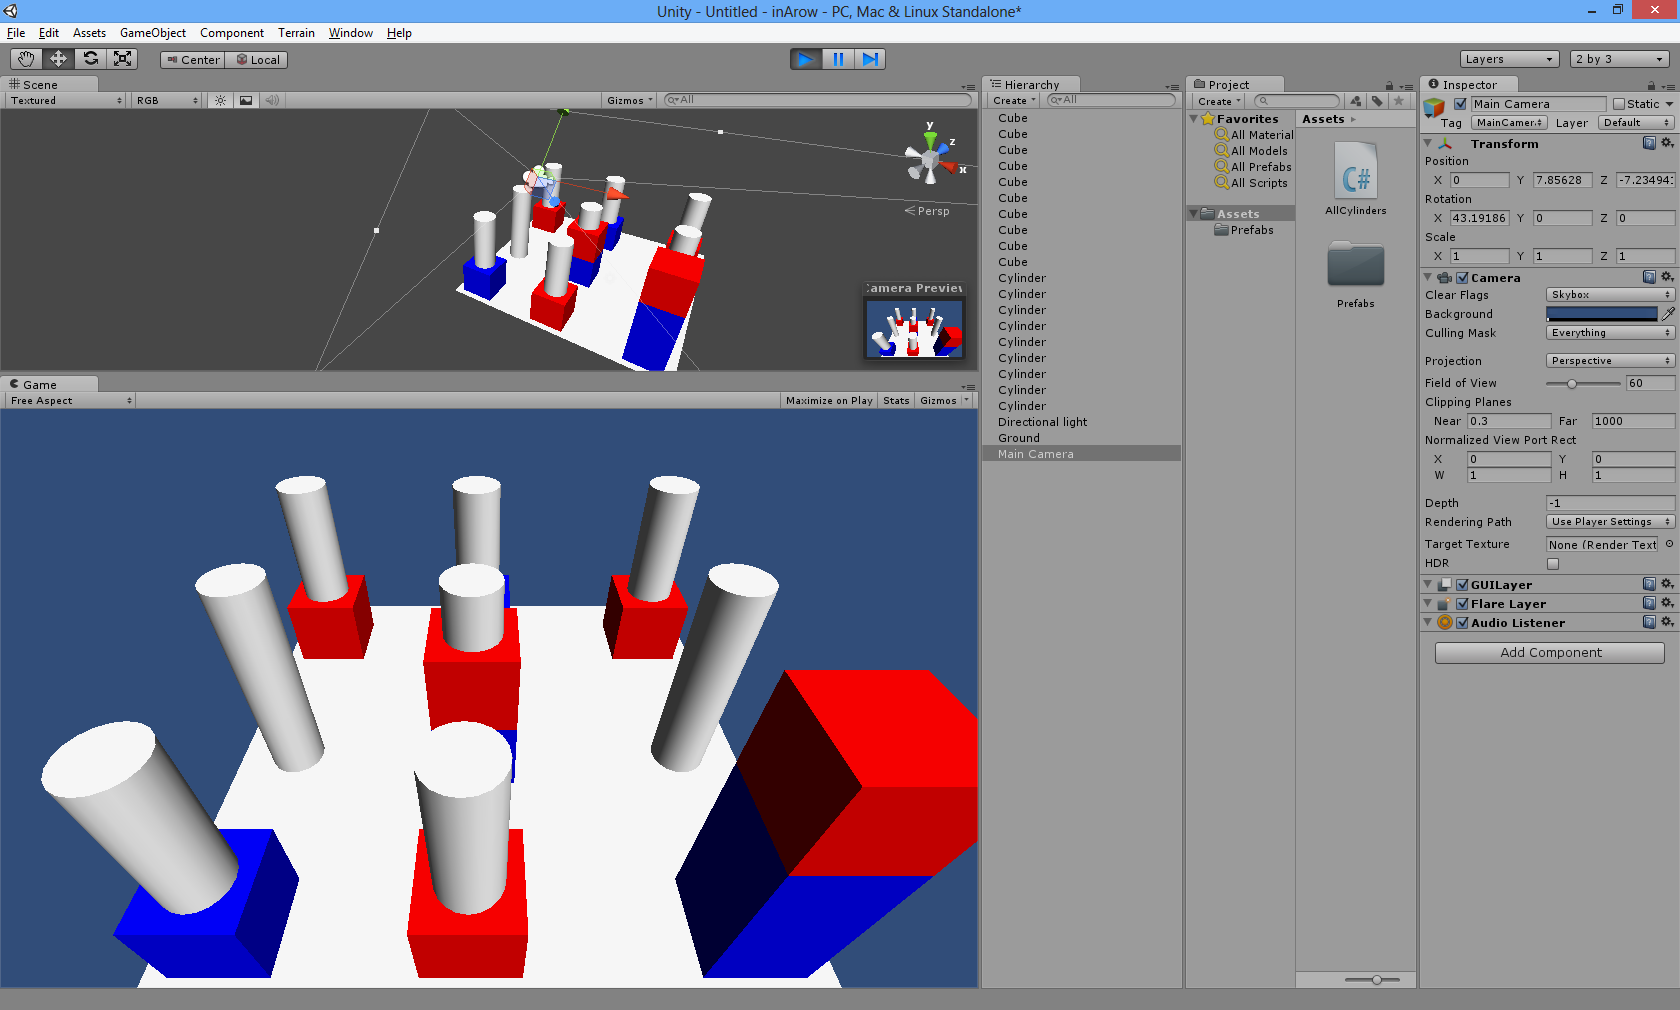
\includegraphics[width=12cm]{pic/min-editor.png}
\end{center}
\caption{Razvoj grafično intenzivne aplikacije v okolju Unity.}
\label{mineditor}
\end{figure} 

Slika \ref{minplay} prikazuje delovanje aplikacije na mobilni platformi Nexus 7.

\begin{figure}
\begin{center}
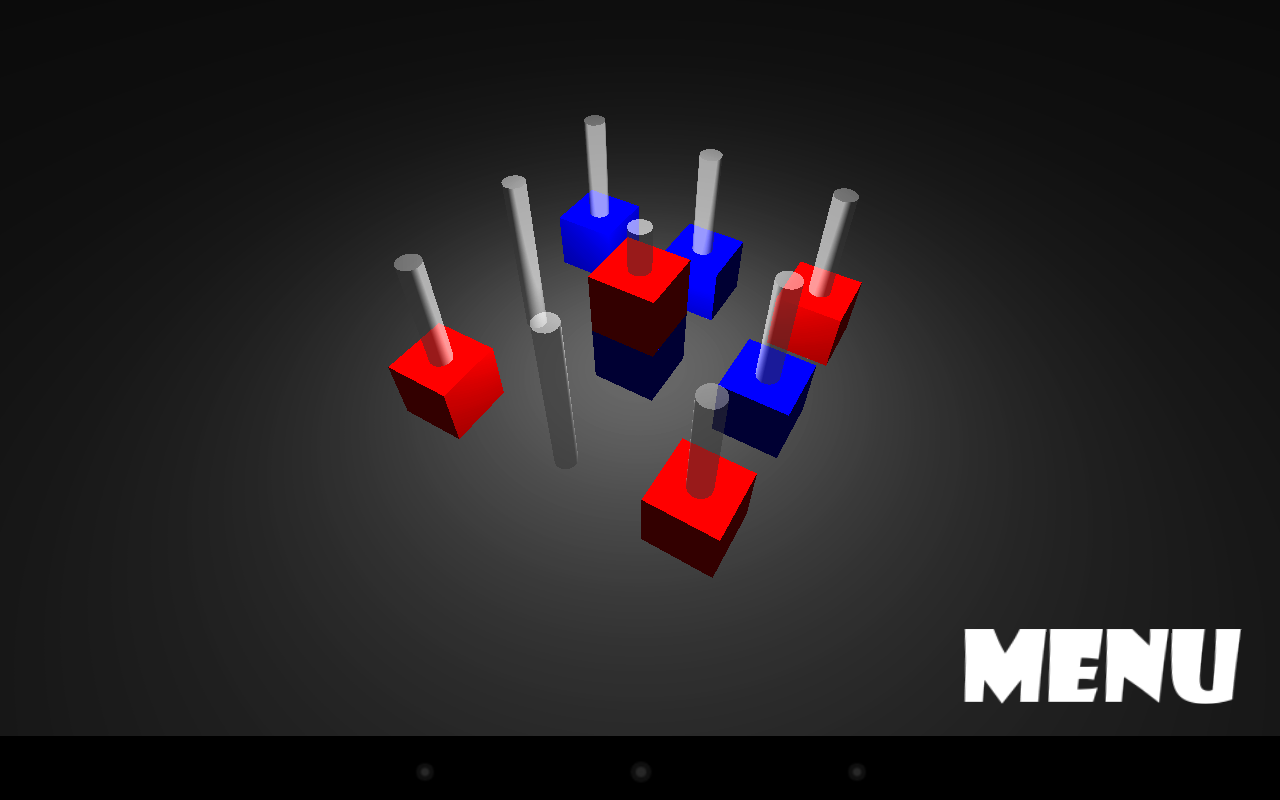
\includegraphics[width=10cm]{pic/min-play.png}
\end{center}
\caption{Končana Unity aplikacija izvožena na mobilno platformo.}
\label{minplay}
\end{figure} 

%\section{Primer C++}

%\section{Primer MIN}

%Primer Min je bil narejen s pomočjo knjižnice LibGDX. Za svoje delovanje izrablja %zmoglivosti OpenGL ES 2.0. 


